%%%%%%%%%%%%%%%%%%%%%%%%%%%%%%%%%%%%%%%%%%%%%%%%%%%%%%%%%%%%%%%%%%%%%%%%
%                                                                      %
%     File: Thesis_Practical_Applications.tex                          %
%     Tex Master: Thesis.tex                                           %
%                                                                      %
%     Author: João C. Godinho                                          %
%     Last modified : Apr 2018                                         %
%                                                                      %
%%%%%%%%%%%%%%%%%%%%%%%%%%%%%%%%%%%%%%%%%%%%%%%%%%%%%%%%%%%%%%%%%%%%%%%%

\chapter{Practical Applications}
\label{chapter:practical_applications}

We take this chapter to briefly describe how we took the previously defined model to the real world, providing practical implementations for it.
The following work is still on-going as part of a scholarship provided by INOV - Inesc Inovação, as such the end products are still being developed and test.

%%%%%%%%%%%%%%%%%%%%%%%%%%%%%%%%%%%%%%%%%%%%%%%%%%%%%%%%%%%%%%%%%%%%%%%%
\section{Malware Detection Service}
\label{section:malware_service}

Our first practical application for the obtained model comes as a malware detection service.
The idea is to take advantage of Cuckoo~\cite{tool:cuckoo} to implement a web service identical to Malwr~\cite{tool:malwr}, but also adding the malware detection by applying our model.

To implement this service, we developed a simple web application that receives files from users and then sends them to a Cuckoo instance running on a server.
We created a custom signature for Cuckoo that takes the analysis results and converts it into features suitable for our model, which is then used to classify the sample.
The output of the model is then appended as a signature the final report.
After analysis our web application extracts basic information regarding the file, as well as the output of the classifier.

Figure \ref{fig:malware_detetor} shows the service being tested with a \texttt{petya}\footnote{Symantec - Petya Ransomware, October 27, 2017 [https://www.symantec.com/blogs/threat-intelligence/petya-ransomware-wiper]} sample, using early versions of our $\LR$ model.

\begin{figure}[!h]
	\centering
	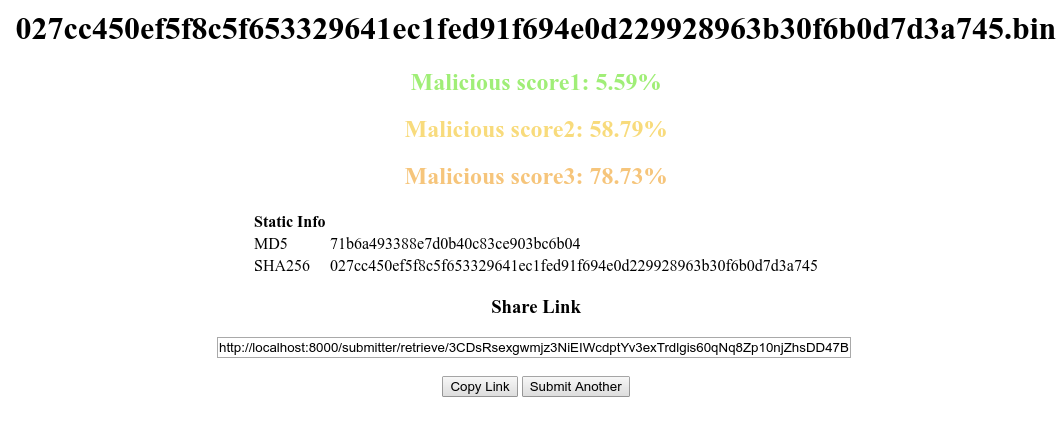
\includegraphics[width=0.8\textwidth]{Figures/malware_detector.png}
	\caption{Malware Detector in early stages.}
	\label{fig:malware_detetor}
\end{figure}

We are currently testing and optimizing the service, as it is not currently using our latest and best model $\mathcal{E}$.

%%%%%%%%%%%%%%%%%%%%%%%%%%%%%%%%%%%%%%%%%%%%%%%%%%%%%%%%%%%%%%%%%%%%%%%%
\section{Email Attachment Scanner}
\label{section:email_scanner}

Our second practical application uses the previous service, but in an automated way, to scan email attachments arriving and departing Inesc's mail server.
The idea is to insert the malware detector in the mail server pipeline as a scanner.

Inesc's mail server uses MailScanner~\cite{tool:mailscanner} to filter and scan emails.
In Figure \ref{fig:mailscanner} we provide a diagram on the MailScanner pipeline.

Our implementation works by creating a custom \textit{Virus Scanner}, which takes email attachments and sends them to the previous described malware detection service.
Upon receiving the results, our custom scanner modifies the mail object to include the classification results.

Further down in the \textit{Message Processing} step, we added a custom step to modify an unused \texttt{Header} in the email to include the classification results.

Currently we are in the process of moving the developed code into the mail server to start obtaining real world results.

\begin{figure}[!h]
	\centering
	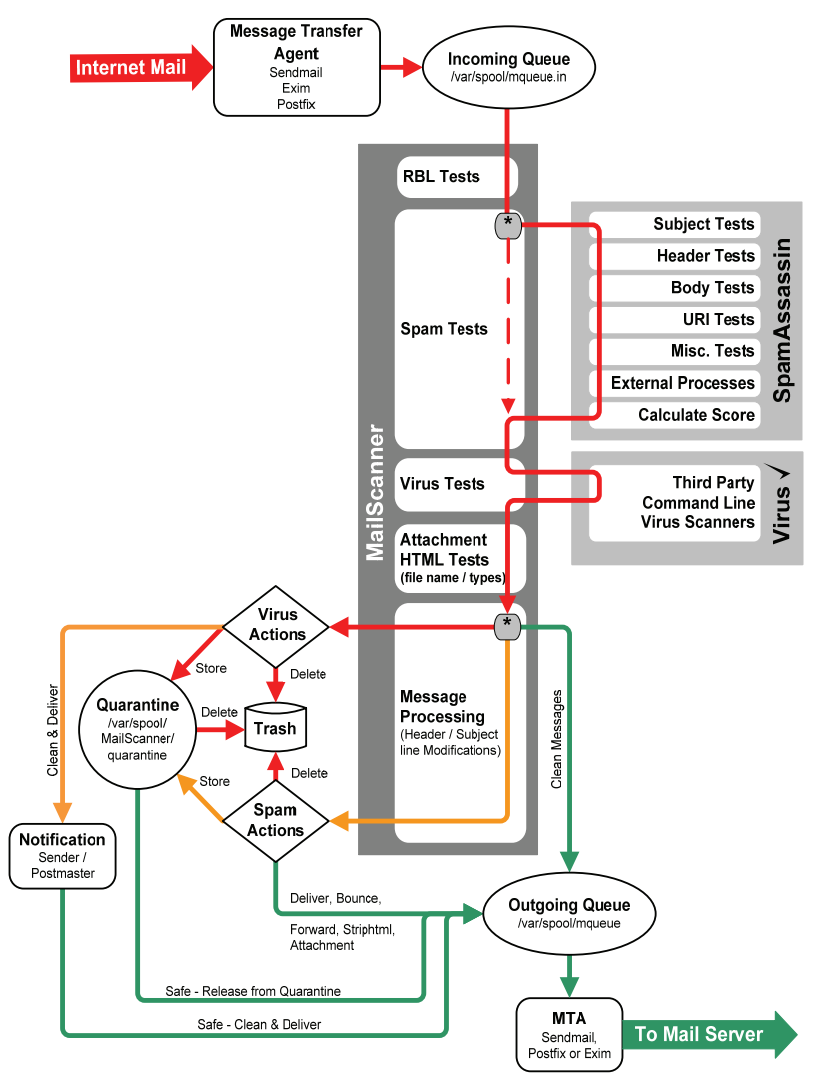
\includegraphics[width=0.8\textwidth]{Figures/mailscanner.png}
	\caption{MailScanner process diagram.}
	\label{fig:mailscanner}
\end{figure}